\documentclass{llncs}
\usepackage{amssymb}
\setcounter{tocdepth}{3}
\usepackage[dvipdfmx]{graphicx}
\usepackage{tikz}
\usepackage{amsmath}
\usepackage{docmute}
\usetikzlibrary{automata}
\usetikzlibrary{arrows}
\usetikzlibrary{positioning}
\usepackage{here}
\usepackage{enumitem}
\usepackage{wrapfig}
\usetikzlibrary{decorations.markings}
\DeclareMathOperator*{\argmin}{arg\,min}

\title{Bit bifurcation by cotranscriptional folding\thanks{This work is in part supported by JST Program to Disseminate Tenure Tracking System, MEXT, Japan, No. 6F36 and JSPS Grant-in-Aid for Young Scientists (A) No. 16H05854 to S.~S.}}
\author{Yusei Masuda \and Shinnosuke Seki\thanks{Corresponding author} \and Yuki Ubukata}
\institute{
Department of Computer and Network Engineering, 
The University of Electro-Communications, 
1-5-1, Chofugaoka, Chofu, Tokyo, 1828585, Japan \email{s.seki@uec.ac.jp}
}

\begin{document}

\maketitle

\begin{abstract}
We demonstrate cotranscriptional folding of a finite part of the Heighway dragon, a fractal also-known as the paperfolding sequence $P = LLRLLRRL \cdots$ by an oritatami system. 
The $i$-th element of $P$ can be obtained by feeding $i$ in binary to a 4-state deterministic finite automaton with output (DFAO). 
We implement this DFAO and a bit-string bifurcator as modules of oritatami system. 
Combining them with a known binary counter module yields the target oritatami system. 
%
\begin{keywords}
Heighway dragon, 
Fractal, 
Cotranscriptional folding, 
Oritatami system, 
Automatic sequence, 
Bitstring bifurcation
\end{keywords}
\end{abstract}

%%%%%%%%%%%%%%%%%%%%%%%%%%%%%%%%%%%%%%%%%%%%%%%%%%%%%%%%%%%%%%%%%%%%%
\subsection{Verificaion}
%%%%%%%%%%%%%%%%%%%%%%%%%%%%%%%%%%%%%%%%%%%%%%%%%%%%%%%%%%%%%%%%%%%%%

We explain the correctness of the folding.
The folding of each module depends on its environment, i.e. on the components already folded nearby and on the current minimum energy conformations output by previous step.
Algorithm~\ref{alg:dragon} is an algorithm of designing the $n$-th iteration of the Heighway dragon.
It shows all possible environments of each module and component.
Using the simulator developed for \cite{HaKiOtSe2016}, we have verified that all of the components fold correctly in all possible environments.


\begin{algorithm}                      
\caption{The $n$-th iteration of the Heighway dragon}         
\label{alg:dragon}                          
\begin{algorithmic}                  
\REQUIRE $n \geq , length \leq 0$

\STATE $current \Leftarrow 0$
\WHILE{$current < 2^n - 1$}

%%%%%%%%%%%%%%%%%%%Counter-zig%%%%%%%%%%%%%%%%%%%
\STATE $carry = 1$
\FOR{$i = 1$ to $n$}
\IF{$carry = 1$}

\IF{above component is body-rpx-0}
\STATE Cozig-11 is folded.
\STATE $carry \Leftarrow 0$ 
\ELSIF{above component is body-rpx-1}
\STATE Cozig-10 is folded.
\ENDIF

\ELSIF{$carry = 0$}

\IF{above component is body-rpx-0}
\STATE Cozig-00 is folded.
\ELSIF{above component is body-rpx-1}
\STATE Cozig-01 is folded.
\ENDIF
\ENDIF
\STATE Spacer is folded.
\ENDFOR

\IF{$carry =1$}
\STATE the folding stops (counter capacity exceeded)
\ENDIF
%%%%%%%%%%%%%%%%%%%Counter-zig%%%%%%%%%%%%%%%%%%%
 
\STATE $current \Leftarrow current + 1$
\ENDWHILE

\end{algorithmic}
\end{algorithm}

%-------------------------------------------------------------------------------------------
			\subsubsection{Turning module}
%-------------------------------------------------------------------------------------------

\begin{figure}[t]
\centering
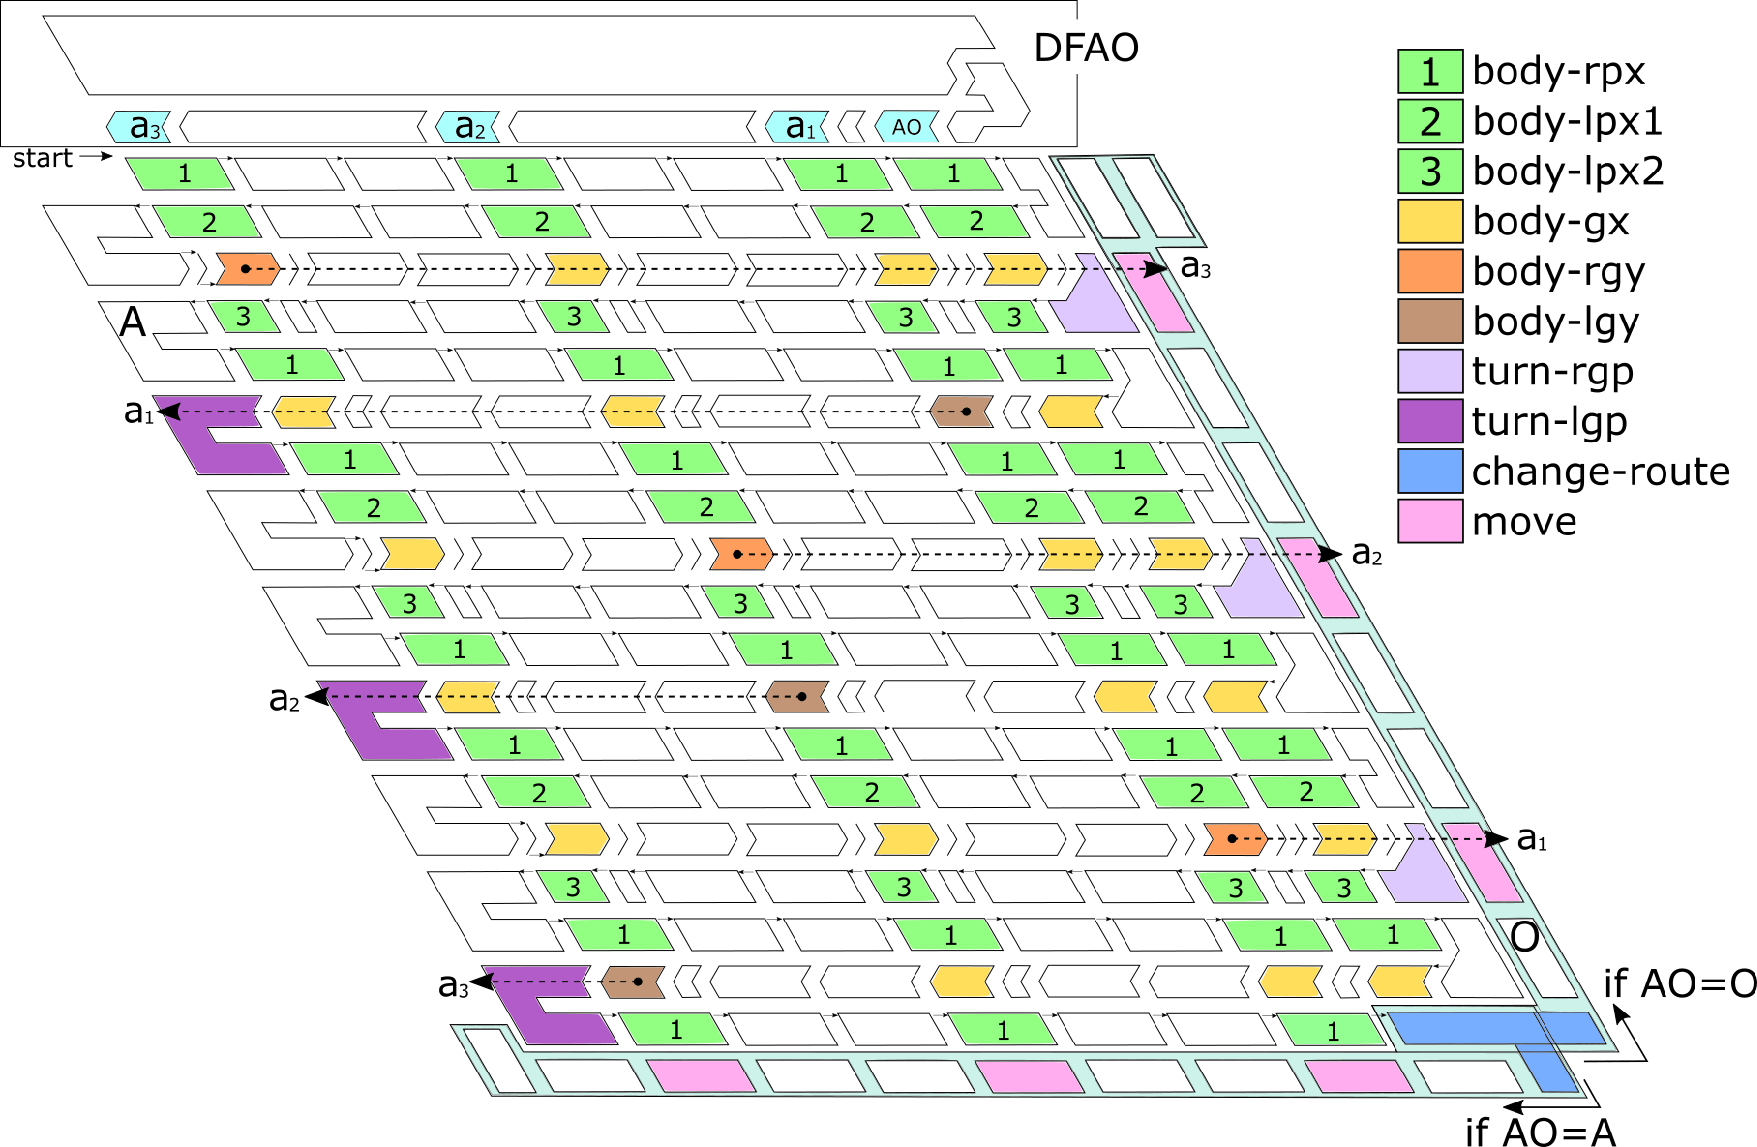
\includegraphics[width=\linewidth]{pic/overall_turn_part.pdf}
\caption{
Component-level abstraction of folding of turning module.
All the white components in the middle are spacers, some of which are implemented in the shape of parallelogram instead of glider. 
 }
\label{fig:overall_turning}
\end{figure}

The last module is for turn. 
It consists of two submodules: bit-sequence bifurcator and steering arm (shaded in light blue in Fig.~\ref{fig:overall_turning}). 

The bifurcator bifurcates the bits of the current count $i$ and the reinterpreted signal (A or O) as shown in Fig.~\ref{fig:abst_dragon} while folding into zigzags.
For that, it employs components to handle the following four types of tasks: 
\begin{enumerate}[itemsep=0pt]
\item propagate 1-bit vertically: body-rpx (Fig.~\ref{fig:body-rpx} (left)), body-lpx1 (Fig.~\ref{fig:body-rpx} (right)), and body-lpx2 (Fig.~\ref{fig:half-adder});
\item let 1-bit cross another 1-bit: body-gx (Fig.~\ref{fig:DFAO-zag2}); 
\item fork 1-bit vertically and horizontally: body-rgy (Fig.~\ref{fig:DFAO-zag2}) and body-lgy (Fig.~\ref{fig:body-lgy});  
\item undergo transition between a zig and a zag and exposes 1-bit outside: turn-rgp (Fig.~\ref{fig:turn-rgp}) and turn-lgp (Fig.~\ref{fig:turn-lgp}). 
\end{enumerate} 
%that propagates 1bit vertically (body-rpx, body-lpx1, and body-lpx2 in Figure~\ref{fig:overall_turning}), that lets 1bit cross another 1bit (body-gx), that forks 1bit vertically and horizontally (body-rgy, body-lgy), and that undergoes transition from a zig to a zag or from a zag to a zig and exposes 1bit outside (turn-rgp, turn-lgp).
Components to handle the first two types of tasks have already been implemented (see, e.g., \cite{HaKiOtSe2016}) so that we shall explain the others.

%The component body-rgy takes one of the two conformations in Figure~\ref{fig:body-rgy} depending on the 1-bit encoded in the two beads above.
%Output below, the 1-bit is encoded as a type of the second bead from left, while output right, it is encoded as the position of its last bead (top or bottom).
%Its zag-variant, body-lgy, is implemented analogously; for its conformations.

%\begin{figure}[h]
\begin{wrapfigure}{r}{0.55\linewidth}
\vspace*{-5mm}
\centering
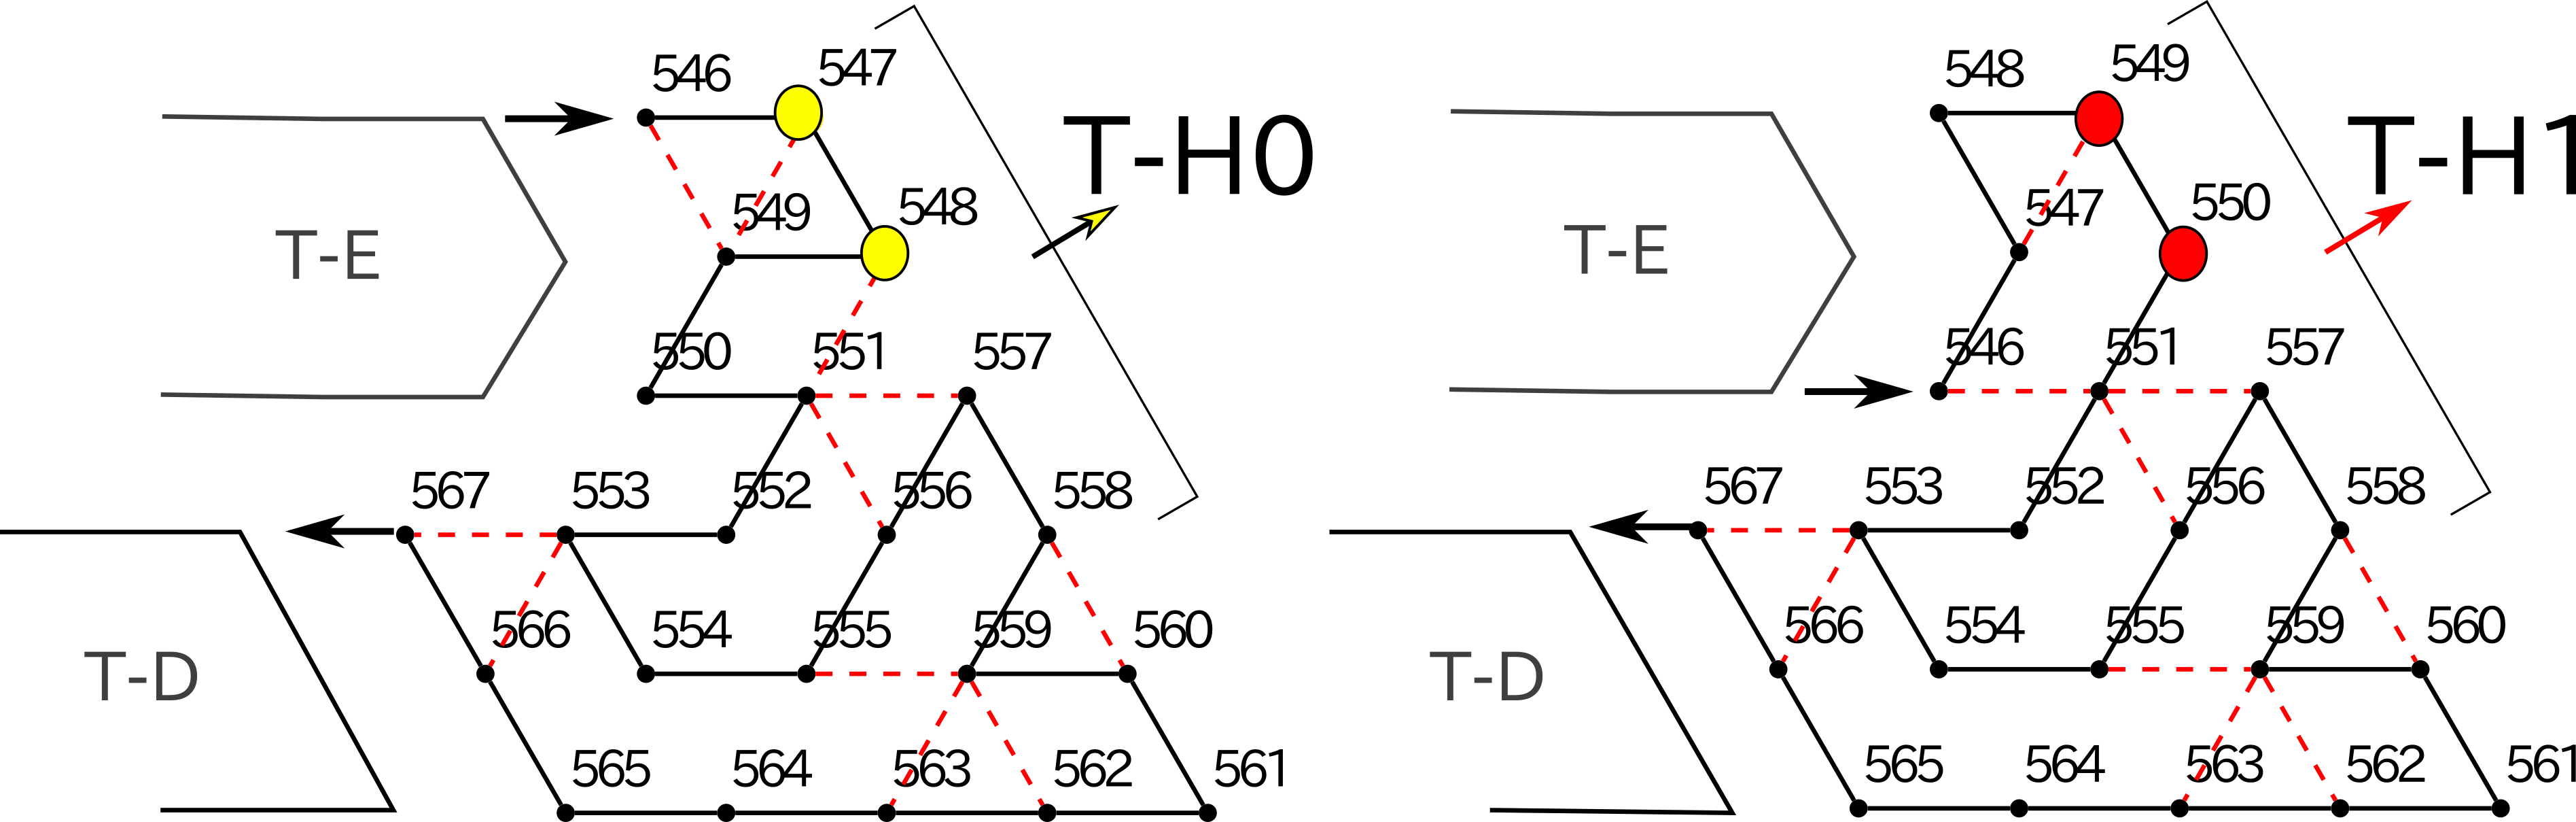
\includegraphics[width=\linewidth]{pic/turn-rgp.png}
\caption{The two conformations of turn-rgp.}
\label{fig:turn-rgp}
\vspace*{-3mm}
\end{wrapfigure}
%\end{figure}

The component body-rgy is implemented by reusing the first half of DFAO-zag2 (Fig.~\ref{fig:DFAO-zag2}). 
Starting from the bottom, it can take two conformations which end at different heights and expose sequences of bead types sufficiently pairwise distinct downward. 
Hence, we can divert it to fork 1bit input rightward and downward. 
The 1bit thus forked transfers till the end of a zag and is converted by the turn-rgp into a sequence of bead types (see Fig.~\ref{fig:turn-rgp}). 
The body-lgy and turn-lgp are their zig counterparts (Figs.~\ref{fig:body-lgy} and \ref{fig:turn-lgp}). 

%The 1bit forked rightward by a body-rgy transfers till the end of the zig without being jammed because all remaining modules in the zig are designed in such a way that they start and end at the same height like the even-distance glider.
%The module turn-rgp receives the 1bit (top or bottom), and exposes it by taking one of the two comformations in Figure~\ref{fig:turn-rgp}.
%The module turn-lgp functions analogously in zags as being folded in Figure~\ref{fig:turn-lgp}.

\begin{figure}[h]
\centering
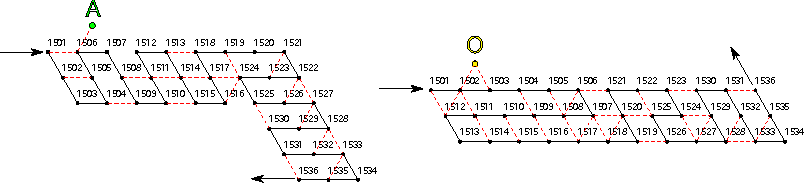
\includegraphics[width=\linewidth]{pic/change_route.pdf}
\caption{The two conformations of change-route.}
\label{fig:change_route}
\end{figure}

The bifurcator also propagates the 1-bit A/O, output by the DFAO module, to tell the steering arm which way it should take.
Specifically, the signal has the component, change-route, of the steering arm take one of the two conformations in Fig.~\ref{fig:change_route}, guiding the rest of the arm towards the specified direction.
The remaining arm is a catenation of move components (Fig.~\ref{fig:move}), which is capable of letting the bifurcated bit sequence through.  
Note that the turning module need not bifurcate AO.
Indeed, the second and third turning modules are supposed to turn in the same manner as the first one.
It hence suffices to append A and O to the bifurcated bit sequences on the acute side and obtuse side, respectively, as shown in Fig.~\ref{fig:overall_turning}.

\begin{remark}
As suggested in Fig.~\ref{fig:overall_turning}, the bifurcation component actually outputs an input bit sequence also downward.
That is, it trifurcates the input.
This provides a more space-efficient way to replicate a bit sequence many-folds.
\end{remark}


\section*{Appendix}
\subsection{Turner}
Turner consists of two parts: bit string bifurcator and steering arm (colored in blue in Fig.~\ref{over_all}).
%steering arm
\begin{figure}[t]
 \centering
\scalebox{0.45}{
 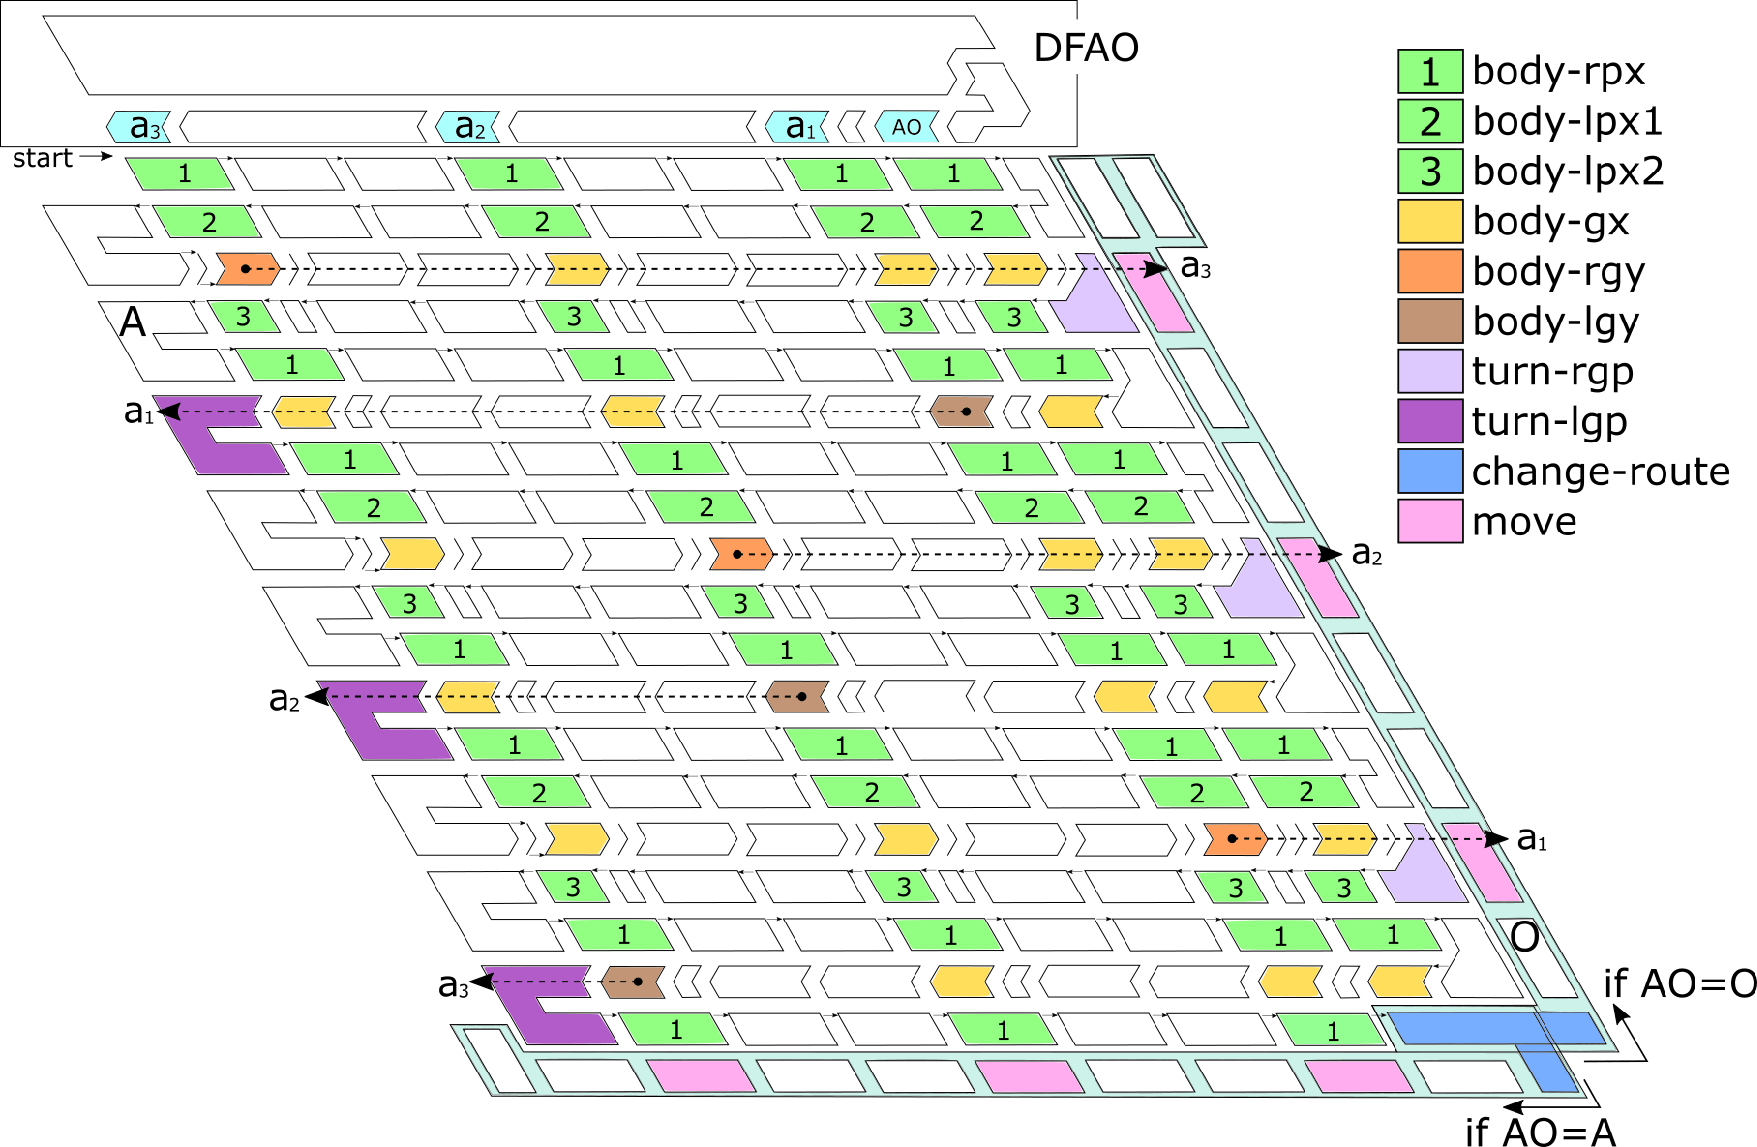
\includegraphics{pic/overall_turn_part.pdf}
}
 \caption{The module-level abstraction of folding of Turner.
 All the white modules in the middle are spacers, some of which are implemented in the shape of parallelogram instead of glider. 
 %Note that the steering arm, colored in blue here, folds upward if AO = O or leftward otherwise, though both of them are drawn in here.
 }
\label{over_all}
\end{figure}

The bifurcator sends binary information as in Fig.~\ref{fig:abst_dragon} while folding into zigzags.
For that, it employs four types of module that propagates 1bit vertically (body-rpx, body-lpx1, and body-lpx2 in Fig.~\ref{over_all}), that lets 1bit cross another 1bit (body-gx), that forks 1bit vertically and horizontally (body-rgy, body-lgy), and that undergoes transition from a zig to a zag or from a zag to a zig and exposes 1bit outside (turn-rgp, turn-lgp).
The first two of them have already been implemented (see, e.g., \cite{HaKiOtSe2016}) so that we shall explain the others.

\begin{figure}[t]
 \centering
\scalebox{1}{
 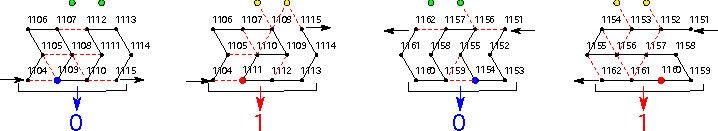
\includegraphics[width=\linewidth]{pic/body_rlgy.pdf}
}
 \caption{(left) The possible two conformations of body-rgy and (right) of body-lgy.}
\label{body-y}
\end{figure}

The module body-rgy takes one of the two conformations in Fig.~\ref{body-y} (left) depending on the 1bit encoded in the two beads above.
Output below, the 1bit is encoded as a type of the second bead from left, while output right, it is encoded as whether this module ends top or bottom.
Its zag-variant, body-lgy, is implemented analogously; for its conformations, see Fig.~\ref{body-y} (right).

\begin{figure}[t]
 \centering
\scalebox{1}{
 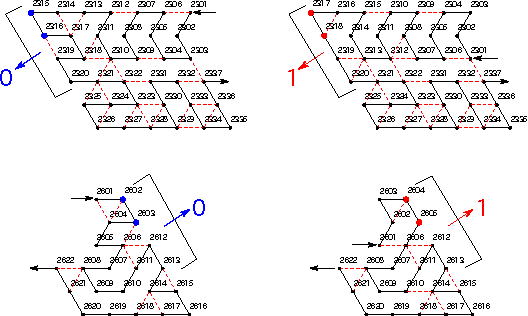
\includegraphics{pic/body_lrgp.pdf}
}
 \caption{(top) The possible two conformations of turn-lgp and (bottom) of turn-rgp.}
\label{turn}
\end{figure}

The 1bit forked rightward by a body-rgy transfers till the end of the zig without being jammed because all remaining modules in the zig are designed in such a way that they start and end at the same height like the glider.
The module turn-rgp receives the 1bit (top or bottom), and exposes it by taking one of the two comformations in Fig.~\ref{turn} (bottom).
The module turn-lgp functions analogously in zags as being holded in Fig.~\ref{turn} (top).

\begin{figure}[t]
 \centering
\scalebox{1}{
 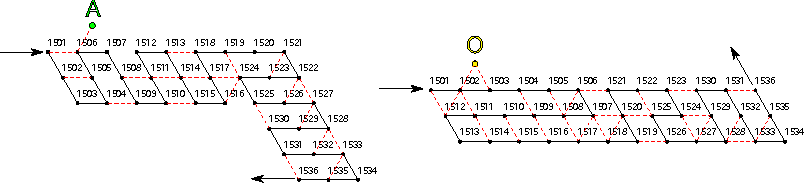
\includegraphics[width=\linewidth]{pic/change_route.pdf}
}
 \caption{The possible two conformations of change-route.}
\label{change_route}
\end{figure}

The bifurcator also propagates a signal, A or O, fed by the DFAO, to tell the steering arm which way it should take.
Specifically, the signal has the first module, change-route, of the steering arm take one of the two conformations in Fig.~\ref{change_route}, guiding the rest of the steering arm in the ordered direction.
The steering arm is provided with move modules, which let the bifurcated bit string pass through.  
Note that the Turner does not have to bifurcate AO.
Indeed, the second Turner is supposed to turn in the same manner as the first one.
It hence suffices to append A and O to the bifurcated bit strings on the acute side and obtuse side, respectively, as shown in Fig.~\ref{over_all}.


\begin{figure}[H]
  \begin{tabular}{c}
 
  
  \begin{minipage}{0.5\hsize}
  \centering
  \scalebox{0.5}{
  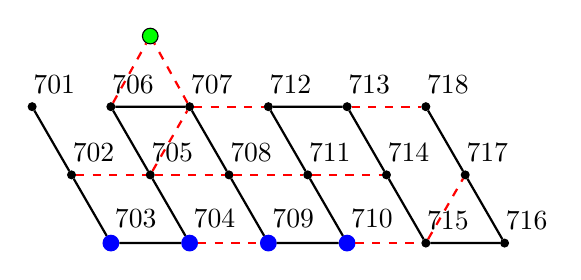
\begin{tikzpicture}[node distance=1cm,every node/.style={draw,circle,fill,inner sep=1pt}]
   \node[blue,inner sep = 2pt] (3) at (0:0)[label=above right:703]{};
  \node (2) at (120:1)[label=above right:702]{};
  \node (1)at (120:2)[label=above right:701]{};
  \node[right of= 1] (6) [label=above right:706]{};
  \node[right of =6](7)[label=above right:707]{};
  \node[right of =7](12)[label=above right:712]{};
\node[right of =12](13)[label=above right:713]{};
\node[right of =13](18)[label=above right:718]{};
  \node[right of =2](5)[label=above right:705]{};
  \node[right of =5](8)[label=above right:708]{};
  \node[right of =8](11)[label=above right:711]{};
\node[right of =11](14)[label=above right:714]{};
\node[right of =14](17)[label=above right:717]{};
  \node[right of =3,blue,inner sep = 2pt](4)[label=above right:704]{};
  \node[right of =4,blue,inner sep = 2pt](9)[label=above right:709]{};
  \node[right of =9,blue,inner sep = 2pt](10)[label=above right:710]{};
\node[right of =10](15)[label=above right:715]{};
\node[right of =15](16)[label=above right:716]{};
\node[above =1.6cm of  5,fill = green,inner sep = 2pt](100){};
  \draw[thick](1)--(2)--(3)--(4)--(5)--(6)--(7)--(8)--(9)--(10)--(11)--(12)--(13)--(14)--(15)--(16)--(17)--(18);
  \draw[dashed,thick,red](2)--(5);
  \draw[dashed,thick,red](5)--(8);
  \draw[dashed,thick,red](4)--(9);
  \draw[dashed,thick,red](5)--(7);
  \draw[dashed,thick,red](6)--(100);
  \draw[dashed,thick,red](7)--(100);
  \draw[dashed,thick,red](7)--(12);
  \draw[dashed,thick,red](8)--(11);
  \draw[dashed,thick,red](11)--(14);
  \draw[dashed,thick,red](10)--(15);
  \draw[dashed,thick,red](13)--(18);
  \draw[dashed,thick,red](15)--(17);
  \end{tikzpicture}
  }

  \end{minipage}

 \begin{minipage}{0.5\hsize}
  \centering
  \scalebox{0.5}{
  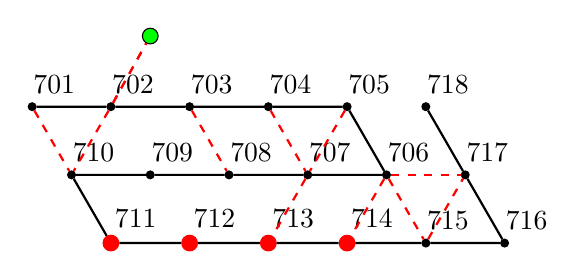
\begin{tikzpicture}[node distance=1cm,every node/.style={draw,circle,fill,inner sep=1pt}]
  \node [red,inner sep = 2pt] (11) at (0:0)[label=above right:711]{};
  \node (10) at (120:1)[label=above right:710]{};
  \node (1)at (120:2)[label=above right:701]{};
  \node[right of= 1] (2) [label=above right:702]{};
  \node[right of =2](3)[label=above right:703]{};
  \node[right of =3](4)[label=above right:704]{};
  \node[right of =4](5)[label=above right:705]{};
  \node[right of =5](18)[label=above right:718]{};
  \node[right of =10](9)[label=above right:709]{};
  \node[right of =9](8)[label=above right:708]{};
  \node[right of =8](7)[label=above right:707]{};
  \node[right of =7](6)[label=above right:706]{};
  \node[right of =6](17)[label=above right:717]{};
  \node[right of =11,red,inner sep = 2pt](12)[label=above right:712]{};
  \node[right of =12,red,inner sep = 2pt](13)[label=above right:713]{};
  \node[right of =13,red,inner sep = 2pt](14)[label=above right:714]{};
  \node[right of =14](15)[label=above right:715]{};
  \node[right of =15](16)[label=above right:716]{};
\node[above =1.6cm of 9,fill = green,inner sep = 2pt](100){};
  \draw[thick](1)--(2)--(3)--(4)--(5)--(6)--(7)--(8)--(9)--(10)--(11)--(12)--(13)--(14)--(15)--(16)--(17)--(18);
  \draw[dashed,thick,red](2)--(100);
  \draw[dashed,thick,red](2)--(100);
  \draw[dashed,thick,red](1)--(10);
  \draw[dashed,thick,red](2)--(10);
  \draw[dashed,thick,red](3)--(8);
  \draw[dashed,thick,red](4)--(7);
  \draw[dashed,thick,red](5)--(7);
  \draw[dashed,thick,red](7)--(13);
  \draw[dashed,thick,red](6)--(14);
  \draw[dashed,thick,red](6)--(15);
  \draw[dashed,thick,red](6)--(17);
  \draw[dashed,thick,red](15)--(17);
  \end{tikzpicture}
  }
 
  \end{minipage}

 \\
  
  \begin{minipage}{0.5\hsize}
  \centering
  \scalebox{0.5}{
  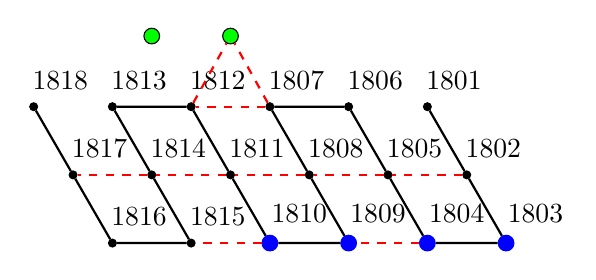
\begin{tikzpicture}[node distance=1cm,every node/.style={draw,circle,fill,inner sep=1pt}]
   \node[blue,inner sep = 2pt] (3) at (0:0)[label=above right:1803]{};
  \node (2) at (120:1)[label=above right:1802]{};
  \node (1)at (120:2)[label=above right:1801]{};
  \node[left of= 1] (6) [label=above right:1806]{};
  \node[left of =6](7)[label=above right:1807]{};
  \node[left of =7](12)[label=above right:1812]{};
\node[left of =12](13)[label=above right:1813]{};
\node[left of =13](18)[label=above right:1818]{};
  \node[left of =2](5)[label=above right:1805]{};
  \node[left of =5](8)[label=above right:1808]{};
  \node[left of =8](11)[label=above right:1811]{};
\node[left of =11](14)[label=above right:1814]{};
\node[left of =14](17)[label=above right:1817]{};
  \node[left of =3,blue,inner sep = 2pt](4)[label=above right:1804]{};
  \node[left of =4,blue,inner sep = 2pt](9)[label=above right:1809]{};
  \node[left of =9,blue,inner sep = 2pt](10)[label=above right:1810]{};
\node[left of =10](15)[label=above right:1815]{};
\node[left of =15](16)[label=above right:1816]{};
\node[above =1.6cm of  11,fill = green,inner sep = 2pt](100){};
\node[above =1.6cm of  14,fill = green,inner sep = 2pt](101){};
  \draw[thick](1)--(2)--(3)--(4)--(5)--(6)--(7)--(8)--(9)--(10)--(11)--(12)--(13)--(14)--(15)--(16)--(17)--(18);
  \draw[dashed,thick,red](2)--(5);
  \draw[dashed,thick,red](5)--(8);
  \draw[dashed,thick,red](8)--(11);
  \draw[dashed,thick,red](11)--(14);
  \draw[dashed,thick,red](14)--(17);
  \draw[dashed,thick,red](4)--(9);
  \draw[dashed,thick,red](7)--(12);
  \draw[dashed,thick,red](10)--(15);
  \draw[dashed,thick,red](7)--(100);
  \draw[dashed,thick,red](12)--(100);
  \end{tikzpicture}
  }
  \end{minipage}

 \begin{minipage}{0.5\hsize}
  \centering
  \scalebox{0.5}{
  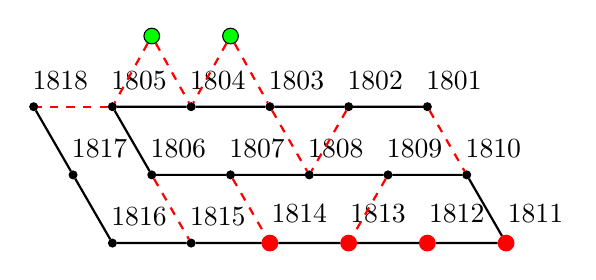
\begin{tikzpicture}[node distance=1cm,every node/.style={draw,circle,fill,inner sep=1pt}]
  \node [red,inner sep = 2pt] (11) at (0:0)[label=above right:1811]{};
  \node (10) at (120:1)[label=above right:1810]{};
  \node (1)at (120:2)[label=above right:1801]{};
  \node[left of= 1] (2) [label=above right:1802]{};
  \node[left of =2](3)[label=above right:1803]{};
  \node[left of =3](4)[label=above right:1804]{};
  \node[left of =4](5)[label=above right:1805]{};
  \node[left of =5](18)[label=above right:1818]{};
  \node[left of =10](9)[label=above right:1809]{};
  \node[left of =9](8)[label=above right:1808]{};
  \node[left of =8](7)[label=above right:1807]{};
  \node[left of =7](6)[label=above right:1806]{};
  \node[left of =6](17)[label=above right:1817]{};
  \node[left of =11,red,inner sep = 2pt](12)[label=above right:1812]{};
  \node[left of =12,red,inner sep = 2pt](13)[label=above right:1813]{};
  \node[left of =13,red,inner sep = 2pt](14)[label=above right:1814]{};
  \node[left of =14](15)[label=above right:1815]{};
  \node[left of =15](16)[label=above right:1816]{};
\node[above =1.6cm of 6,fill = green,inner sep = 2pt](100){};
\node[above =1.6cm of 7,fill = green,inner sep = 2pt](101){};
  \draw[thick](1)--(2)--(3)--(4)--(5)--(6)--(7)--(8)--(9)--(10)--(11)--(12)--(13)--(14)--(15)--(16)--(17)--(18);
  \draw[dashed,thick,red](1)--(10);
  \draw[dashed,thick,red](2)--(8);
  \draw[dashed,thick,red](3)--(8);
  \draw[dashed,thick,red](9)--(13);
  \draw[dashed,thick,red](7)--(14);
  \draw[dashed,thick,red](6)--(15);
  \draw[dashed,thick,red](5)--(18);
  \draw[dashed,thick,red](100)--(5);
  \draw[dashed,thick,red](100)--(4);
  \draw[dashed,thick,red](101)--(4);
  \draw[dashed,thick,red](101)--(3);
  \end{tikzpicture}
  }
  \end{minipage}
 
\\

  \begin{minipage}{0.5\hsize}
  \centering
  \scalebox{0.5}{
  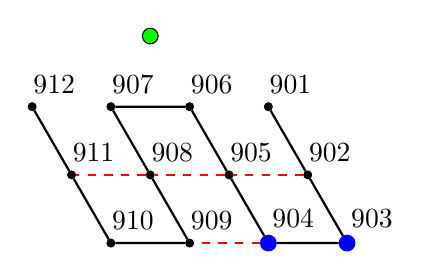
\begin{tikzpicture}[node distance=1cm,every node/.style={draw,circle,fill,inner sep=1pt}]
  \node (3) at (0:0) [blue,inner sep =2pt,label=above right:903]{};
  \node (2) at (120:1)[label=above right:902]{};
  \node (1)at (120:2)[label=above right:901]{};
  \node[left of= 1] (6) [label=above right:906]{};
  \node[left of =6](7)[label=above right:907]{};
  \node[left of =7](12)[label=above right:912]{};
  \node[left of =2](5)[label=above right:905]{};
  \node[left of =5](8)[label=above right:908]{};
  \node[left of =8](11)[label=above right:911]{};
  \node[left of =3](4)[blue,inner sep = 2pt,label=above right:904]{};
  \node[left of =4,](9)[label=above right:909]{};
  \node[left of =9](10)[label=above right:910]{};
  

\node[above =1.6cm of  8,fill = green,inner sep = 2pt](100){};
  \draw[thick](1)--(2)--(3)--(4)--(5)--(6)--(7)--(8)--(9)--(10)--(11)--(12);
  \draw[dashed,thick,red](2)--(5);
  \draw[dashed,thick,red](5)--(8);
  \draw[dashed,thick,red](8)--(11);
  \draw[dashed,thick,red](4)--(9);
  \end{tikzpicture}
  }
  
  \end{minipage}

 \begin{minipage}{0.5\hsize}
  \centering
  \scalebox{0.5}{
  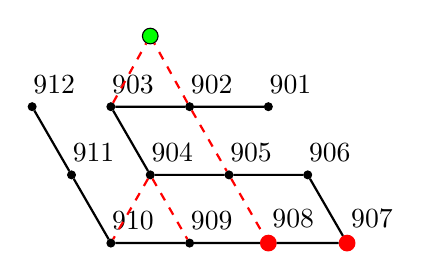
\begin{tikzpicture}[node distance=1cm,every node/.style={draw,circle,fill,inner sep=1pt}]
  \node (7) at (0:0)[red,inner sep = 2pt,label=above right:907]{};
  \node (6) at (120:1)[label=above right:906]{};
  \node (1)at (120:2)[label=above right:901]{};
  \node[left of= 1] (2) [label=above right:902]{};
  \node[left of =2](3)[label=above right:903]{};
  \node[left of =3](12)[label=above right:912]{};
  \node[left of =6](5)[label=above right:905]{};
  \node[left of =7,red,inner sep = 2pt](8)[label=above right:908]{};
  \node[left of =8](9)[label=above right:909]{};
  \node[left of =9](10)[label=above right:910]{};
  \node[left of =5](4)[label=above right:904]{};
  \node[left of =4](11)[label=above right:911]{};
  
\node[above =1.6cm of 4,fill = green,inner sep = 2pt](100){};

  \draw[thick](1)--(2)--(3)--(4)--(5)--(6)--(7)--(8)--(9)--(10)--(11)--(12);
  \draw[dashed,thick,red](2)--(5);
  \draw[dashed,thick,red](5)--(8);
  \draw[dashed,thick,red](4)--(9);
  \draw[dashed,thick,red](4)--(10);
  \draw[dashed,thick,red](2)--(100);
  \draw[dashed,thick,red](3)--(100);
  \end{tikzpicture}
  }
  
  \end{minipage}
  \end{tabular}
  \caption{%body-lpx2
(top) The possible two conformations of body-rpx, (middle) The possible two conformations of body-lpx1, (bottom) The possible two conformations of body-lpx2.}
\label{body-px}
\end{figure} 


\begin{figure}[H]
  \begin{tabular}{c}
  \begin{minipage}{0.25\hsize}
  \centering
  \scalebox{0.5}{
  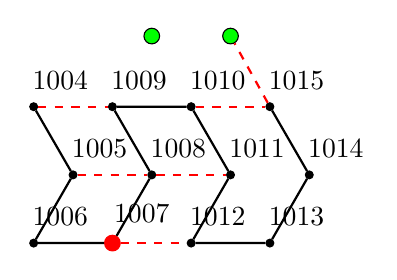
\begin{tikzpicture}[node distance=1cm,every node/.style={draw,circle,fill,inner sep=1pt}]
  \node (3) at (0:0)[label=above right:1006]{};
  \node (2) at (60:1)[label=above right:1005]{};
  \node (6)at (60:2)[label=above right:1009]{};
  \node[right of =3,red,inner sep = 2pt](4)[label=above right:1007]{};
  \node[right of =4](9)[label=above right:1012]{};
  \node[right of =9](10)[label=above right:1013]{};
  
  \node[right of =2](5)[label=above right:1008]{};
  \node[right of =5](8)[label=above right:1011]{};
  \node[right of =8](11)[label=above right:1014]{};
  
  \node[left of= 6] (1) [label=above right:1004]{};
  \node[right of =6](7)[label=above right:1010]{};
  \node[right of =7](12)[label=above right:1015]{};
  \node[above =1.6cm of 8,fill = green,inner sep = 2pt](100){};
  \node[above =1.6cm of 5,fill = green,inner sep = 2pt](101){};
  \draw[thick](1)--(2)--(3)--(4)--(5)--(6)--(7)--(8)--(9)--(10)--(11)--(12);
  \draw[dashed,thick,red](1)--(6);
  \draw[dashed,thick,red](2)--(5);
  \draw[dashed,thick,red](4)--(9);
  \draw[dashed,thick,red](5)--(8);
  \draw[dashed,thick,red](7)--(12);
  \draw[dashed,thick,red](12)--(100);
  \end{tikzpicture}
  }
  
  \end{minipage}

\begin{minipage}{0.25\hsize}
  \centering
  \scalebox{0.5}{
  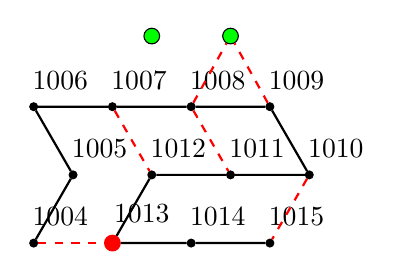
\begin{tikzpicture}[node distance=1cm,every node/.style={draw,circle,fill,inner sep=1pt}]
  \node (1) at (0:0)[label=above right:1004]{};
  \node (2) at (60:1)[label=above right:1005]{};
  \node (4)at (60:2)[label=above right:1007]{};
  \node[left of= 4] (3) [label=above right:1006]{};
  \node[right of =4](5)[label=above right:1008]{};
    \node[right of =5](6)[label=above right:1009]{};
    \node[right of =2](9)[label=above right:1012]{};
    \node[right of =9](8)[label=above right:1011]{};
    \node[right of =8](7)[label=above right:1010]{};
    \node[right of =1,red,inner sep = 2pt](10)[label=above right:1013]{};
    \node[right of =10](11)[label=above right:1014]{};
    \node[right of =11](12)[label=above right:1015]{};
  
  \node[above =1.6cm of 8,fill = green,inner sep = 2pt](100){};
\node[above =1.6cm of 9,fill = green,inner sep = 2pt](101){};
  \draw[thick](1)--(2)--(3)--(4)--(5)--(6)--(7)--(8)--(9)--(10)--(11)--(12);
  \draw[dashed,thick,red](4)--(9);
  \draw[dashed,thick,red](5)--(8);
  \draw[dashed,thick,red](7)--(12);
  \draw[dashed,thick,red](1)--(10);
  \draw[dashed,thick,red](5)--(100);
  \draw[dashed,thick,red](6)--(100);
  \end{tikzpicture}
  }
 
  \end{minipage}

\begin{minipage}{0.25\hsize}
  \centering
  \scalebox{0.5}{
  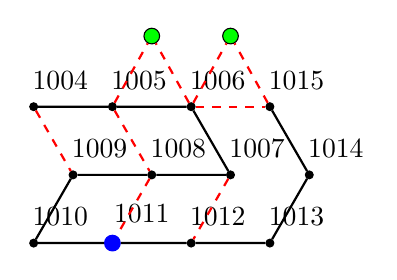
\begin{tikzpicture}[node distance=1cm,every node/.style={draw,circle,fill,inner sep=1pt}]
  \node (1) at (0:0)[label=above right:1004]{};
  \node (6) at (-60:1)[label=above right:1009]{};
  \node (8)at (-60:2)[blue,inner sep = 2pt,label=above right:1011]{};
 \node[left of= 8] (7) [label=above right:1010]{};
  \node[right of =1](2)[label=above right:1005]{};
  \node[right of =2](3)[label=above right:1006]{};
  \node[right of =6](5)[label=above right:1008]{};
  \node[right of =5](4)[label=above right:1007]{};
  \node[right of =8](9)[label=above right:1012]{};
  \node[right of =9](10)[label=above right:1013]{};
  \node[right of =3](12)[label=above right:1015]{};
  \node[right of =4](11)[label=above right:1014]{};
  
 
  \node[above =1.6cm of 4,fill = green,inner sep = 2pt](100){};
\node[above =1.6cm of 5,fill = green,inner sep = 2pt](101){};
  
  \draw[thick](1)--(2)--(3)--(4)--(5)--(6)--(7)--(8)--(9)--(10)--(11)--(12);
  \draw[dashed,thick,red](1)--(6);
  \draw[dashed,thick,red](2)--(5);
  \draw[dashed,thick,red](5)--(8);
  \draw[dashed,thick,red](4)--(9);
  \draw[dashed,thick,red](3)--(12);
  \draw[dashed,thick,red](2)--(101);
  \draw[dashed,thick,red](3)--(101);
  \draw[dashed,thick,red](3)--(100);
  \draw[dashed,thick,red](12)--(100);
  \end{tikzpicture}
  }
  
  \end{minipage}


\begin{minipage}{0.25\hsize}
  \centering
  \scalebox{0.5}{
  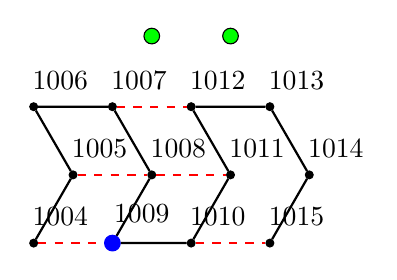
\begin{tikzpicture}[node distance=1cm,every node/.style={draw,circle,fill,inner sep=1pt}]
  \node (3) at (0:0)[label=above right:1006]{};
  \node (2) at (-60:1)[label=above right:1005]{};
  \node (6)at (-60:2)[blue,inner sep = 2pt,label=above right:1009]{};
  \node[right of =3](4)[label=above right:1007]{};
  \node[right of =4](9)[label=above right:1012]{};
  \node[right of =9](10)[label=above right:1013]{};
  
  \node[right of =2](5)[label=above right:1008]{};
  \node[right of =5](8)[label=above right:1011]{};
  \node[right of =8](11)[label=above right:1014]{};
  
  \node[left of= 6] (1) [label=above right:1004]{};
  \node[right of =6](7)[label=above right:1010]{};
  \node[right of =7](12)[label=above right:1015]{};

  \node[above =1.6cm of 8,fill = green,inner sep = 2pt](){};
\node[above =1.6cm of 5,fill = green,inner sep = 2pt](){};
  \draw[thick](1)--(2)--(3)--(4)--(5)--(6)--(7)--(8)--(9)--(10)--(11)--(12);
  \draw[dashed,thick,red](1)--(6);
  \draw[dashed,thick,red](7)--(12);
  \draw[dashed,thick,red](2)--(5);
  \draw[dashed,thick,red](5)--(8);
  \draw[dashed,thick,red](4)--(9);
  \end{tikzpicture}
  }
 
  \end{minipage}
  \end{tabular}
  \caption{The possible four conformations of body-gx.}
\label{body-gx}
\end{figure} 



\begin{figure}[H]
  \begin{tabular}{c}
 
  
  \begin{minipage}{0.5\hsize}
  \centering
  \scalebox{0.5}{
  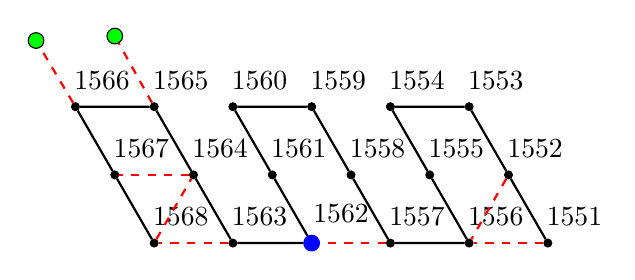
\begin{tikzpicture}[node distance=1cm,every node/.style={draw,circle,fill,inner sep=1pt}]
   \node (1) at (0:0)[label=above right:1551]{};
  \node (2) at (120:1)[label=above right:1552]{};
  \node (3)at (120:2)[label=above right:1553]{};
  \node[left of= 1] (6) [label=above right:1556]{};
  \node[left of =6](7)[label=above right:1557]{};
  \node[left of =7,blue,inner sep = 2pt](12)[label=above right:1562]{};
\node[left of =12](13)[label=above right:1563]{};
\node[left of =13](18)[label=above right:1568]{};
  \node[left of =2](5)[label=above right:1555]{};
  \node[left of =5](8)[label=above right:1558]{};
  \node[left of =8](11)[label=above right:1561]{};
\node[left of =11](14)[label=above right:1564]{};
\node[left of =14](17)[label=above right:1567]{};
  \node[left of =3](4)[label=above right:1554]{};
  \node[left of =4](9)[label=above right:1559]{};
  \node[left of =9](10)[label=above right:1560]{};
\node[left of =10](15)[label=above right:1565]{};
\node[left of =15](16)[label=above right:1566]{};
\coordinate[left of = 17](99){};
\node[above =1.6cm of  17,fill = green,inner sep = 2pt](100){};
\node[above =1.6cm of  99,fill = green,inner sep = 2pt](101){};
  \draw[thick](1)--(2)--(3)--(4)--(5)--(6)--(7)--(8)--(9)--(10)--(11)--(12)--(13)--(14)--(15)--(16)--(17)--(18);
  \draw[dashed,thick,red](1)--(6);
  \draw[dashed,thick,red](2)--(6);
\draw[dashed,thick,red](7)--(12);
\draw[dashed,thick,red](13)--(18);
\draw[dashed,thick,red](18)--(14);
\draw[dashed,thick,red](14)--(17);
\draw[dashed,thick,red](16)--(101);
\draw[dashed,thick,red](15)--(100);
  \end{tikzpicture}
  }
  \end{minipage}

 \begin{minipage}{0.5\hsize}
  \centering
  \scalebox{0.5}{
  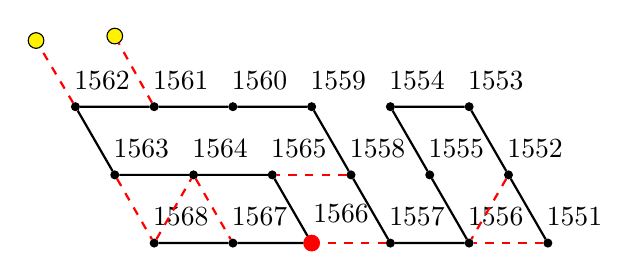
\begin{tikzpicture}[node distance=1cm,every node/.style={draw,circle,fill,inner sep=1pt}]
   \node (1) at (0:0)[label=above right:1551]{};
  \node (2) at (120:1)[label=above right:1552]{};
  \node (3)at (120:2)[label=above right:1553]{};
  \node[left of= 1] (6) [label=above right:1556]{};
  \node[left of =6](7)[label=above right:1557]{};
  \node[left of =7,red,inner sep = 2pt](16)[label=above right:1566]{};
\node[left of =16](17)[label=above right:1567]{};
\node[left of =17](18)[label=above right:1568]{};
  \node[left of =2](5)[label=above right:1555]{};
  \node[left of =5](8)[label=above right:1558]{};
  \node[left of =8](15)[label=above right:1565]{};
\node[left of =15](14)[label=above right:1564]{};
\node[left of =14](13)[label=above right:1563]{};
  \node[left of =3](4)[label=above right:1554]{};
  \node[left of =4](9)[label=above right:1559]{};
  \node[left of =9](10)[label=above right:1560]{};
\node[left of =10](11)[label=above right:1561]{};
\node[left of =11](12)[label=above right:1562]{};
\coordinate[left of = 13](99){};
\node[above =1.6cm of  13,fill = yellow,inner sep = 2pt](100){};
\node[above =1.6cm of  99,fill = yellow,inner sep = 2pt](101){};
  \draw[thick](1)--(2)--(3)--(4)--(5)--(6)--(7)--(8)--(9)--(10)--(11)--(12)--(13)--(14)--(15)--(16)--(17)--(18);
  \draw[dashed,thick,red](1)--(6);
\draw[dashed,thick,red](2)--(6);
\draw[dashed,thick,red](8)--(15);
\draw[dashed,thick,red](7)--(16);
\draw[dashed,thick,red](13)--(18);
\draw[dashed,thick,red](18)--(14);
\draw[dashed,thick,red](14)--(17);
\draw[dashed,thick,red](12)--(101);
\draw[dashed,thick,red](11)--(100);
  \end{tikzpicture}
  }
  \end{minipage}
 
 \end{tabular}
  \caption{The possible two conformations of move.}
\label{move}
\end{figure} 
\begin{remark}
In fact, as suggested in Fig.~\ref{over_all}, the bifurcator outputs the bit string also downward.
That is, it bifurcates a given bit string into three directions.
This provides a more space-efficient way to replicate a bit string many-folds.
\end{remark}

\bibliographystyle{splncs03}
\bibliography{dna23}

\end{document}


